\documentclass[11pt]{article}
\usepackage[margin=0.8in]{geometry}
\usepackage{graphicx}
\usepackage{booktabs}
\usepackage{hyperref}
\usepackage{xurl}
\usepackage{amsmath}
\usepackage{array}
\usepackage{xcolor}
\usepackage{caption}
\usepackage{placeins}
\captionsetup{font=small}

\title{PLC Ligand-Conditioned Binding-Residue Prediction Report}
\author{PLC project internal group-meeting report}
\date{2026-07-07}

\begin{document}
\maketitle

\section*{Executive Summary}
This report summarizes the current PLC project status for ligand-conditioned protein binding-residue prediction.
The current working model family is built around a stable protein trunk, late ligand-conditioned local delta, and controlled protein-gradient feedback.
Across V11m6/V11m6n and later probes, the most consistent empirical conclusion is that useful ligand-conditioned residue localization comes primarily from ligand graph structure and local atom chemistry (\texttt{local54}), while global molecular descriptors and UniMol-style priors are weak contributors in the present heads.

On the PDBbind-style internal ligand-dependency evaluation, the protected no-gate V11m6n line gives real test F1 around 0.606--0.608 with a stable real-shuffle gap of about 0.08.
The best V11m6n grad-scale probe is \texttt{grad060\_no\_gate}, with validation best F1=0.5882 and test real F1=0.6082.
Later V13 residue-atom bias and value-enrichment probes mostly preserve the same ligand-dependency profile but do not improve over the V11m13 group-rescompat baseline; therefore V13 scalar/pair-bias variants are not the current mainline.

The strongest recent benchmark direction is the ESM3 global-prior scratch line.
Across seeds 43--46, ESM3 scratch improves HOLO4K over ESM3 full-finetune in sample F1, PDR, LAA, boundary F1, and protein-level aggregates.
The current benchmark means are: HOLO4K sample F1=0.3482$\pm$0.0058, PDR=0.5193$\pm$0.0116, LAA=0.1739$\pm$0.0029, and BP-F1=0.7820$\pm$0.0073.
COACH420 remains easier in the full per-ligand benchmark, but the HOLO4K gap is largely driven by multi-ligand and large/multimer cases rather than uniform failure: single-ligand HOLO4K proteins are close to COACH420 single-ligand proteins.

\section*{Dataset, Preprocessing, and QC}
The external benchmark branch currently focuses on COACH420 and HOLO4K from the P2Rank benchmark universe.
The local benchmark preparation includes fixed heavy-residue PDBs, protein V4 feature extraction, ligand V5 feature extraction, per-ligand contact/near tags, ESM2 features, and ESM3 latent features.
The current benchmark ESM3 feature cache is complete for the fixed benchmark PDB set:

\begin{table}[t]
\centering
\caption{Current local benchmark feature/QC coverage.}
\begin{tabular}{lrr}
\toprule
Artifact & COACH420 & HOLO4K \\
\midrule
Fixed heavy-residue PDBs & 420 & 4009 \\
Raw ESM3 latent files & 420 & 4009 \\
Normalized ESM3 latent files & 420 & 4009 \\
\bottomrule
\end{tabular}
\end{table}

ESM3 features were extracted locally and normalized with the training-set ESM3 statistics in \path{data/stats/esm3_stats_output.pt}.
The current per-ligand benchmark uses \texttt{max\_atoms=-1}; this removes the earlier ligand atom-count cap and evaluates each protein-ligand row independently.
For a protein with multiple ligands, e.g. $A$ paired with ligands $B,C,D,E$, the per-ligand benchmark creates rows $A$--$B$, $A$--$C$, $A$--$D$, and $A$--$E$.
Each row uses the same protein graph but the current ligand feature and the current ligand-specific residue tag.
This is stricter than aggregate pocket detection because the model must assign the correct pocket to the current ligand.

\begin{figure}[t]
  \centering
  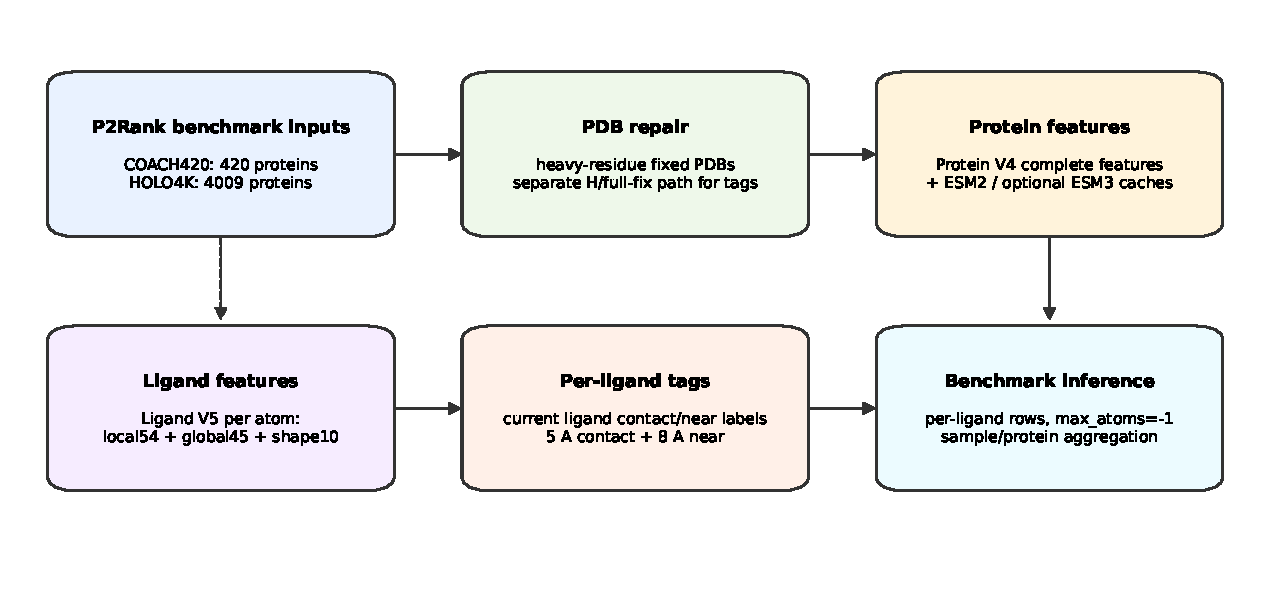
\includegraphics[width=0.98\linewidth]{figures/fig_qc_pipeline.pdf}
  \caption{PLC preprocessing and benchmark-QC flow. The benchmark path separates fixed protein structures, ligand features, per-ligand tags, normalized ESM3 features, and final per-ligand/no-atom-cap inference.}
\end{figure}
\FloatBarrier

\section*{Feature Engineering: Protein Complete V4 and Ligand V5}
The current input design is deliberately asymmetric.
The protein side provides a strong residue-level structural prior, while the ligand side provides atom-local chemical evidence and ligand graph structure.
This matters for interpreting the ablations: the model is not asked to discover residue geometry from ligand features alone; instead, ligand evidence modulates an already strong protein decision space.

\begin{figure}[t]
  \centering
  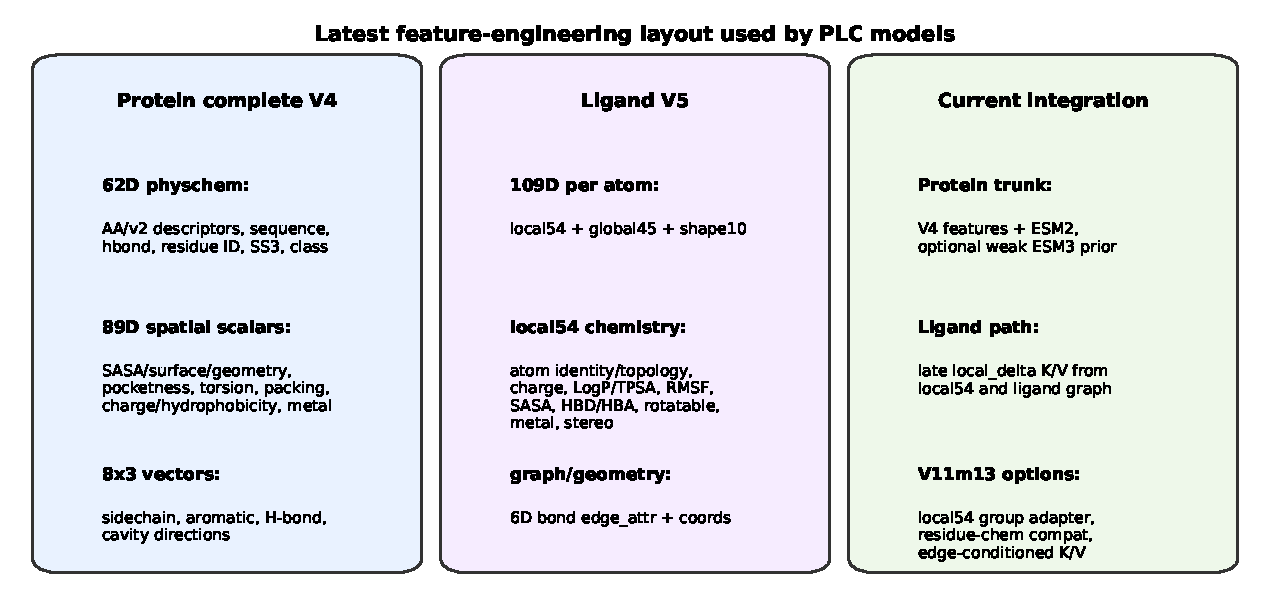
\includegraphics[width=0.98\linewidth]{figures/fig_feature_engineering.pdf}
  \caption{Latest PLC feature-engineering layout. Protein complete V4 supplies residue physicochemical, scalar geometry, and directional vector features. Ligand V5 supplies local atom chemistry, global molecular tags, shape descriptors, graph edges, and coordinates. V11m13-style heads primarily use local54/graph evidence through late local-delta K/V paths.}
\end{figure}

\begin{table}[t]
\centering
\caption{Protein complete feature V4 decomposition.}
\resizebox{\linewidth}{!}{%
\begin{tabular}{lll}
\toprule
Block & Shape & Contents \\
\midrule
Physicochemical & $N_{\mathrm{res}}\times 62$ & V2 residue descriptors, sequence context, H-bond features, 20-way residue identity, SS3, and coarse residue class \\
Spatial scalar & $N_{\mathrm{res}}\times 89$ & SASA/surface, structural geometry, pocketness/flexibility/environment, local density, center distance, surface normal, charge/hydrophobicity, torsions, side-chain packing, environment composition, metal-binding potential, and anisotropy \\
Spatial vector & $N_{\mathrm{res}}\times 8\times 3$ & Side-chain base and COM directions, aromatic normal, H-bond donor/acceptor directions, and multi-scale cavity pointing vectors at 6/10/14 A \\
Metadata & per residue/protein & Residue names, residue indices, chain IDs, CA coordinates, all-atom metadata, sequence, feature version, and spatial scalar feature names \\
\bottomrule
\end{tabular}%
}
\end{table}

The protein V4 scalar geometry block is normalized with train-set statistics when available.
The current benchmark path uses the same protein feature contract as training:
\path{physchem_features}, \path{spatial_scalar_features}, \path{spatial_vector_features}, coordinates, and residue metadata.
ESM2 and ESM3 features are not replacements for this complete feature set; they are additional protein priors attached to the same residue indexing.

\begin{table}[t]
\centering
\caption{Ligand V5 feature decomposition.}
\resizebox{\linewidth}{!}{%
\begin{tabular}{lll}
\toprule
Block & Shape & Contents \\
\midrule
Local atom chemistry & $N_{\mathrm{atom}}\times 54$ & 33D base atom identity/topology plus Gasteiger charge, Crippen LogP contribution, TPSA contribution, RMSF/flexibility, atom SASA, lipophilic SASA, HBD/HBA flags, chirality flags, rotatable-bond context, metal-binding flags, and stereochemistry flags \\
Global molecular tag & $N_{\mathrm{atom}}\times 45$ & PyPropel global molecular descriptor broadcast to each atom \\
Shape features & $N_{\mathrm{atom}}\times 10$ & Normalized 3D shape/inertial/principal-axis descriptors broadcast to each atom \\
Graph and coordinates & edges / coordinates & \texttt{edge\_index}, 6D \texttt{edge\_attr} for bond type/aromaticity/conjugation/ring, current coordinates, and heavy-atom coordinates \\
\bottomrule
\end{tabular}%
}
\end{table}

Thus the final ligand atom feature is 109D:
\[
109 = 54_{\mathrm{local}} + 45_{\mathrm{global}} + 10_{\mathrm{shape}}.
\]
The current source ablations show that the effective residue-localization signal is dominated by local54 and ligand graph edges.
Global45/global55-style molecular descriptors and UniMol-like priors are therefore treated as weak priors or calibration signals, not as the main route for residue assignment.

\section*{Training Data and Splits}
The internal training/evaluation task is a PDBbind-style protein-ligand pair problem.
Each training row contains one protein graph, one ligand graph, and residue-level contact/near labels for that specific ligand.
This is a \emph{per-ligand} formulation, not an aggregate pocket-label formulation: if the same protein structure is paired with multiple ligands, the current ligand determines the positive residue mask for that row.

Training and validation use train-set statistics for continuous feature normalization, including protein spatial scalar features and ESM3 latent features when ESM3 is enabled.
The benchmark path mirrors this rule by normalizing COACH420/HOLO4K ESM3 features with \path{data/stats/esm3_stats_output.pt} and by using the training feature-stat file \path{data/stats/stats_output.pt}.
This avoids the earlier failure mode where benchmark ESM3 scales were mismatched to the training distribution.

The core internal ligand-dependency test table is computed on 1778 test rows for each run in the current ledger.
The protocol evaluates real paired ligands, shuffled ligands, zero ligands, and source-specific zeroing.
These checks are necessary because a higher real score alone is not enough: if shuffle or zero scores rise in parallel, the model may only have learned a stronger protein prior.
The accepted evidence pattern is higher real F1 together with a preserved real-shuffle gap and interpretable source drops.

\section*{Model Architecture}
The current mainline is best described as a V11m13-style model family.
It keeps a strong protein-side trunk and uses ligand information mainly as a late residual correction, rather than letting ligand fusion replace the residue decision geometry.
The protein stream consumes complete V4 residue features plus ESM priors.
The ESM branch is configurable as ESM2 final-layer features or ESM2 multi-layer cache fusion (\emph{weighted-sum} or \emph{concat-projection}), with ESM3 optionally injected as a weak global protein prior.
The ligand stream consumes V5 atom features and graph edges, then passes local atom chemistry and ligand graph evidence to the late local-delta branch.

\begin{figure}[t]
  \centering
  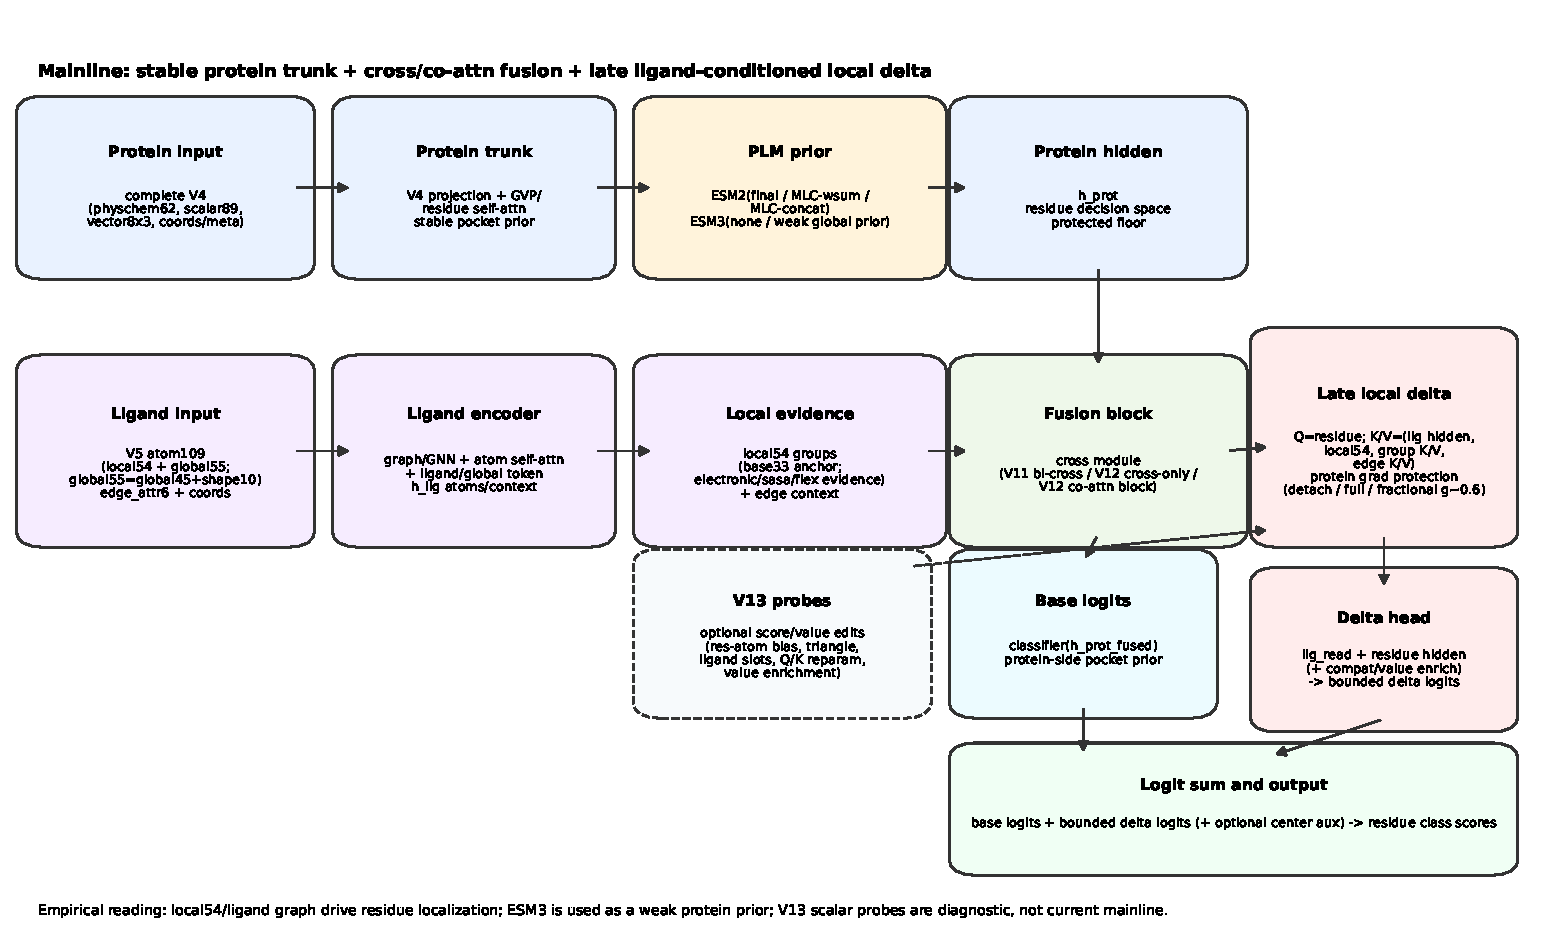
\includegraphics[width=0.99\linewidth]{figures/fig_model_architecture.pdf}
  \caption{Current PLC model architecture. Parentheses mark active alternatives or probes: ESM2 can be final-layer or MLC-based, ESM3 can be absent or used as a weak global prior, and the cross module can be V11 bidirectional cross-attention, V12-style cross-only, or V12-style co-attention. The current strongest line keeps the protein trunk stable and injects ligand evidence through late local-delta K/V paths driven by ligand hidden states, local54 chemistry, local54 group interactions, and edge-conditioned context. V13 residue-atom/triangle/slot/value modules are shown as optional probes, not the current mainline.}
\end{figure}
\FloatBarrier

Operationally, the output is the sum of a protein-side base classifier and a bounded ligand-conditioned delta classifier.
The base classifier protects the protein pocket prior.
The delta branch attends from residues to ligand atoms with residue queries and ligand/local54-derived keys and values.
The protected-gradient setting controls how much the delta loss can update the protein trunk: hard detach is too conservative, full no-detach is fragile, and the current useful region is fractional feedback around \texttt{grad060}.

\section*{Model Evolution and Training Findings}
The V11 line established the main architecture pattern: keep the protein trunk stable, inject ligand evidence late through a local delta path, and avoid letting a complex fusion module replace the protein-side decision geometry.
The key transition from V11m6 to V11m6n was replacing hard detach/full no-detach with fractional protein-gradient feedback.
Full no-detach improves real F1 but can become zero-ligand fragile; fractional gradient preserves ligand awareness while reducing this fragility.

\begin{figure}[t]
  \centering
  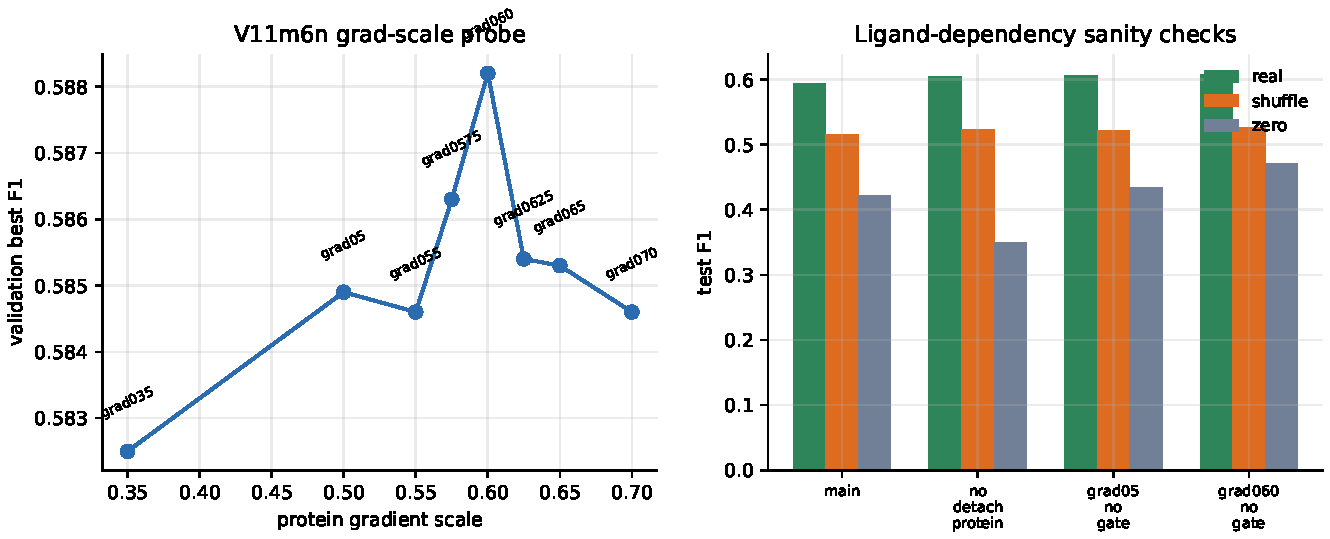
\includegraphics[width=0.98\linewidth]{figures/fig_grad_ligdep.pdf}
  \caption{Left: V11m6n protein-gradient scale probe. The best single probe is around 0.60. Right: ligand-dependency checks; real-shuffle gaps around 0.08 indicate that the paired ligand contributes to residue decisions.}
\end{figure}

\begin{table}[t]
\centering
\caption{V11m6n multi-seed validation summary.}
\begin{tabular}{lrrrr}
\toprule
Seed set & Seeds & Mean best F1 & Std. & Range \\
\midrule
\texttt{grad05\_no\_gate} seed42--46 & 5 & 0.5853 & 0.0027 & 0.5824--0.5885 \\
\texttt{grad060\_no\_gate} seed42--46 & 5 & 0.5864 & 0.0018 & 0.5840--0.5882 \\
\texttt{grad05\_no\_gate} seed43--46 & 4 & 0.5854 & 0.0031 & 0.5824--0.5885 \\
\texttt{grad060\_no\_gate} seed43--46 & 4 & 0.5859 & 0.0017 & 0.5840--0.5879 \\
\bottomrule
\end{tabular}
\end{table}

\section*{Ligand Dependency and Source Ablations}
The ligand-dependency protocol evaluates real paired ligands, shuffled ligands, zero ligands, and feature/source splits.
The main question is whether a higher real score is due to true paired-ligand evidence or merely a stronger protein prior.
The current V11m6n evidence supports true ligand use: \texttt{grad060\_no\_gate} reaches real F1=0.6082 while shuffle drops to 0.5269 and zero drops to 0.4716.

\begin{table}[t]
\centering
\caption{Core test ligand-dependency results. Primary metric is global class-0 F1.}
\resizebox{\linewidth}{!}{%
\begin{tabular}{lrrrrrr}
\toprule
Run & Real & Shuffle & Zero & Real-shuffle & Real-zero & Precision / Recall \\
\midrule
\texttt{main} & 0.5942 & 0.5154 & 0.4225 & 0.0788 & 0.1717 & 0.6110 / 0.5783 \\
\texttt{no\_gate} & 0.6008 & 0.5257 & 0.4553 & 0.0751 & 0.1455 & 0.6108 / 0.5912 \\
\texttt{no\_detach\_protein} & 0.6052 & 0.5229 & 0.3505 & 0.0823 & 0.2547 & 0.6281 / 0.5839 \\
\texttt{grad05\_no\_gate} & 0.6059 & 0.5222 & 0.4338 & 0.0837 & 0.1721 & 0.6337 / 0.5804 \\
\texttt{grad060\_no\_gate} & 0.6082 & 0.5269 & 0.4716 & 0.0813 & 0.1366 & 0.6357 / 0.5830 \\
\bottomrule
\end{tabular}%
}
\end{table}

Source ablations consistently point to ligand graph and local atom chemistry as the effective ligand signals.
For \texttt{grad060\_no\_gate}, zeroing ligand graph drops F1 by 0.1514 and zeroing local54 drops F1 by 0.1465, while global55 and UniMol drops are only 0.0293 and 0.0019.
This is the main reason the next model direction should emphasize local54/graph evidence and avoid making UniMol/global gates control the local delta.

\begin{figure}[t]
  \centering
  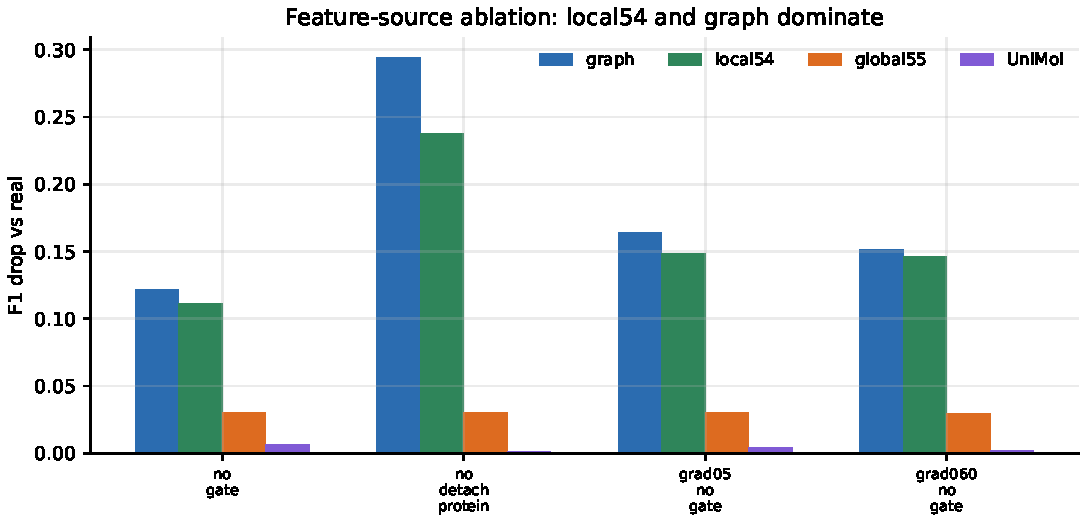
\includegraphics[width=0.78\linewidth]{figures/fig_source_drops.pdf}
  \caption{Feature-source ablation. Local atom chemistry and ligand graph dominate current residue localization; global55 and UniMol provide weak or mostly calibrating signals in the tested heads.}
\end{figure}
\FloatBarrier

\section*{V13 and Protein-Prior Probes}
V13 explored residue-atom scalar bias, triangle-like coherence, slots, value enrichment, and Q/K reparameterization.
The strongest V13 warm-start rows match but do not exceed the V11m13 group-rescompat reference.
For example, \texttt{v13m0\_warm\_resatom\_adapter\_only} has real=0.6157, shuffle=0.5356, zero=0.4473, while the V11m13 group-rescompat reference is real=0.6158, shuffle=0.5355, zero=0.4474.
Scratch V13 variants can increase ligand coupling, with real-shuffle gaps up to about 0.087, but they lose real F1 and become more zero-ligand fragile.

\begin{table}[t]
\centering
\caption{V13 probe summary. Outcomes are judged against the V11m13 group-rescompat reference: real=0.6158, real-shuffle=0.0802, zero=0.4474.}
\resizebox{\linewidth}{!}{%
\begin{tabular}{llll}
\toprule
Probe & How it works & Purpose & Observed outcome \\
\midrule
Residue-atom score bias & Adds a bounded local54-conditioned scalar bias to each residue-atom attention score. & Tests whether atom chemistry can directly correct residue-atom matching. & Warm-start: no effect; scratch co-attn: slight ligand-dependency gain but lower real F1. \\
Triangle/coherence bias & Averages neighboring residues' scores to the same ligand atom and adds a gated residual. & Tests whether local pocket coherence helps suppress isolated attention noise. & Slight real-shuffle gain in scratch co-attn, but real F1 remains below V11m13 and zero fragility increases. \\
Ligand slots & Compresses ligand atoms into learned slot tokens before residue attention. & Tests whether a ligand bottleneck can reduce atom noise and summarize chemistry groups. & No net improvement; co-attn slots preserve real-shuffle but lose real F1 and become zero fragile. \\
Q/K reparameterization & Shifts residue queries and atom keys using ligand context and selected local54 groups. & Tests whether local54 should warp the attention space rather than only add score bias. & Co-attn Q/K reparam gives the largest real-shuffle among V13 probes, but real F1 still drops. \\
Value enrichment & Adds group-specific local54 reads after attention, gated by residue and ligand context. & Tests whether local54 is better used in the value/readout path than in score bias. & Warm-start: no effect; profile matches V11m13 within about 0.0006 F1. \\
Co-attn versus non-coattn & Replaces the V11/V12 cross-only path with a V12-style co-attention block when enabled. & Tests whether self+cross interaction blocks are stronger than cross-only interaction. & Co-attn variants consistently beat non-coattn V13 variants, but V13 still does not beat V11m13. \\
\bottomrule
\end{tabular}%
}
\end{table}

The V13 runs did include co-attention variants.
The V11m8x/V11m13 code path can set \path{use_v12_coattention_block=True} and \path{use_v12_cross_attention=False}; V13 scratch runs explicitly compared co-attn and non-coattn versions.
The observed ordering agrees with the earlier V11 observation that co-attn is stronger than the non-coattn/cross-only path, e.g. V13 co-attn Q/K reparameterization reaches real=0.6070 while the non-coattn counterpart is 0.6016.
However, both remain below the V11m13 group-rescompat reference, so the conclusion is not "co-attn failed"; it is "V13 probe additions did not improve the already-strong co-attn V11m13 basin."

The operational conclusion is that V13 scalar/pair-bias modules should not replace V11m13 as the mainline.
The useful lesson is architectural: richer interaction modules can increase ligand sensitivity, but they must preserve the protein/local54 decision geometry.
The more promising path is protein-side feature fusion and weak global prior injection, which motivated the ESM3 global-prior experiments.

\section*{COACH420/HOLO4K Benchmark Results}
The current external benchmark uses per-ligand evaluation on COACH420 and HOLO4K, with no atom-count cap.
The ESM3 global-prior scratch line is the strongest recent benchmark candidate, particularly on HOLO4K.
Across seeds 43--46, scratch beats full-finetune on HOLO4K in all main metrics.

\begin{figure}[t]
  \centering
  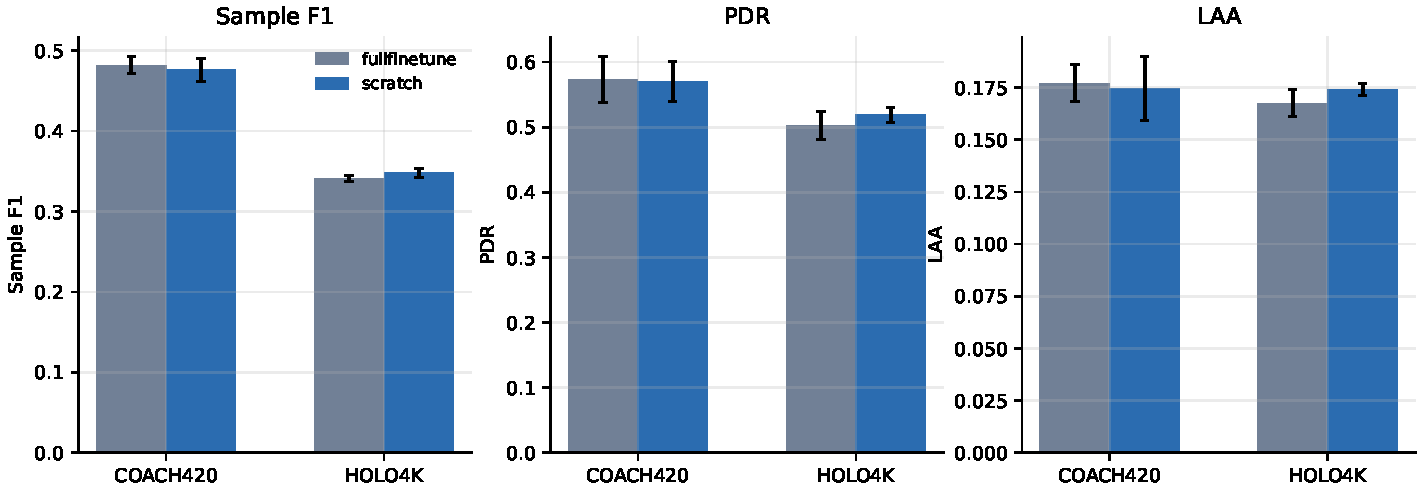
\includegraphics[width=0.98\linewidth]{figures/fig_esm3_benchmark.pdf}
  \caption{ESM3 global-prior benchmark over seeds 43--46. Scratch is consistently better on HOLO4K, especially for PDR, LAA, and boundary F1; full-finetune is slightly higher on COACH420 sample F1 but weaker as a HOLO4K stress-test solution.}
\end{figure}

\begin{table}[t]
\centering
\caption{ESM3 global-prior benchmark summary over seeds 43--46. Values are mean $\pm$ sample std.}
\resizebox{\linewidth}{!}{%
\begin{tabular}{llrrrr}
\toprule
Dataset & Family & Sample F1 & PDR & LAA & BP-F1 \\
\midrule
COACH420 & full-finetune & 0.4819$\pm$0.0106 & 0.5734$\pm$0.0348 & 0.1772$\pm$0.0088 & 0.7637$\pm$0.0069 \\
COACH420 & scratch & 0.4762$\pm$0.0147 & 0.5698$\pm$0.0310 & 0.1746$\pm$0.0153 & 0.7809$\pm$0.0042 \\
HOLO4K & full-finetune & 0.3410$\pm$0.0039 & 0.5028$\pm$0.0219 & 0.1676$\pm$0.0063 & 0.7632$\pm$0.0101 \\
HOLO4K & scratch & \textbf{0.3482$\pm$0.0058} & \textbf{0.5193$\pm$0.0116} & \textbf{0.1739$\pm$0.0029} & \textbf{0.7820$\pm$0.0073} \\
\bottomrule
\end{tabular}%
}
\end{table}
\FloatBarrier

\section*{Why HOLO4K Is Much Lower Than COACH420}
The full HOLO4K per-ligand benchmark is indeed difficult for the current model.
However, the lower score should not be interpreted as a uniform failure on all HOLO4K examples or as evidence that HOLO4K is a predicted-pocket dataset.
The checked P2Rank sources describe HOLO4K as a larger PDB-derived protein-ligand complex benchmark, with more multimer/multi-chain and multi-site cases than COACH420.
P2Rank also notes that PDB-complex-derived ground truth can be incomplete or noisy because not all true binding sites are necessarily occupied by annotated ligands in a given structure.

The most important distinction is between \emph{per-ligand evaluation} and \emph{single-ligand proteins}.
Our per-ligand benchmark decomposes a multi-ligand protein into multiple rows.
But the single-ligand subset used in the gap analysis means proteins with only one annotated ligand in the processed benchmark.
On that subset, HOLO4K is close to COACH420: COACH single-ligand F1 is about 0.548, while HOLO4K single-ligand F1 is about 0.561.
The large overall gap mainly appears when a protein has multiple ligand pockets and the model must perform ligand-specific assignment.

\begin{figure}[t]
  \centering
  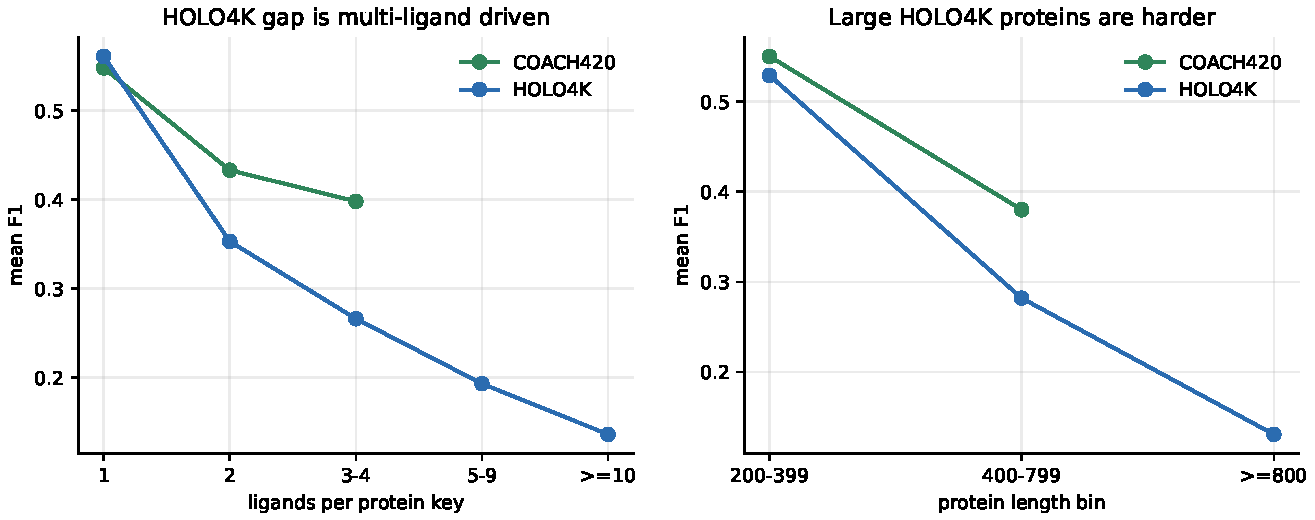
\includegraphics[width=0.98\linewidth]{figures/fig_holo_gap.pdf}
  \caption{HOLO4K gap analysis. Left: single-ligand HOLO4K proteins are close to COACH420; the degradation grows with ligand count. Right: long/multimer-heavy HOLO4K proteins form a harder localization regime.}
\end{figure}

\begin{table}[t]
\centering
\caption{Dataset difficulty statistics from the HOLO4K/COACH420 gap analysis.}
\begin{tabular}{lrrrr}
\toprule
Dataset & Mean residues & Mean contact residues & Mean contact fraction & Multi-ligand rate \\
\midrule
COACH420 & 284 & 16.36 & 0.0686 & 29.0\% \\
HOLO4K & 510 & 16.59 & 0.0485 & 64.8\% \\
\bottomrule
\end{tabular}
\end{table}

For paper writing, the safest interpretation is:
HOLO4K should be treated as a broader stress test for multi-pocket, multi-chain binding-site prediction.
The current model has useful pocket detection and boundary quality, but ligand-specific assignment in multi-ligand proteins remains weak.
This limitation is reflected by the low HOLO4K LAA even when PDR and boundary F1 improve.

\section*{Current Direction and Next Steps}
The current evidence supports three practical directions.
First, keep V11m13/V11-style protected local-delta geometry as the main decision path.
Second, use ESM3 as a weak global protein prior rather than as a heavy replacement for local ligand evidence.
Third, make HOLO4K progress depend on assignment-aware evaluation, not just generic F1.

Near-term experiments should focus on:
\begin{enumerate}
  \item Completing ligand-dependency evaluation for the ESM3 scratch checkpoints to ensure the benchmark gain does not reduce real-shuffle gaps.
  \item Reporting COACH420/HOLO4K metrics stratified by ligand count and protein length.
  \item Developing a lightweight ligand-to-pocket assignment head or ranking calibration that improves multi-ligand HOLO4K LAA without shrinking predicted pockets.
  \item Keeping local54/graph ablations as the primary mechanistic evidence, since global55/UniMol drops remain small.
\end{enumerate}

\section*{Reproducibility Pointers}
Generated report assets are stored under \path{report/data}, \path{report/figures}, and \path{report/scripts}.
The feature-engineering summary used by this report is stored in \path{report/data/feature_engineering_summary.json}.
The ESM3 benchmark summaries were copied from remote completed Slurm jobs into \path{report/data/remote_summaries}.
The V11m6/V11m6n training and ligand-dependency ledgers are archived in \path{report/data/v11m6_v11m6n_experiment_ledger_20260531.md}.
The V13 ligand-dependency summary is archived in \path{report/data/v13_ligdep_9926224_analysis.md}.
The HOLO4K/COACH420 gap analysis is archived in \path{report/data/holo4k_coach420_gap_analysis.md}.

\end{document}
